
\documentclass{scrreprt}

\usepackage[english,ngerman]{babel} 
\usepackage[utf8]{inputenc} 
\usepackage{graphicx}
\usepackage{dsfont}
\usepackage{amsmath}

\title{TH1 - Aufgabenblatt 1}
\author{Andreas Krohn, Erik Andresen, Benjamin Vetter}

\begin{document}

\maketitle

\begin{enumerate}
\item Modelliert einen einfachen Fahrstuhl für 3 Stockwerke, der immer fährt, bis ganz oben (3) und dann wieder bis ganz unten (1).

\item Fügt die Halte-Anforderung für jedes Stockwerk hinzu. Wenn eine Halte-Anforderung vorliegt, hält der Fahrstuhl und die Türen werden geöffnet und vor der Weiterfahrt geschlossen.

\item Modelliert nun einen Fahrstuhl mit einer einfachen Steuerung. Der Fahrstuhl fährt nur, wenn eine Anforderung vorliegt. Falls eine Anforderung für das Stockwerk, in dem sich der Fahrstuhl gerade befindet, vorliegt, werden die Türen geöffnet und anschließend geschlossen. Es wird immer nur eine Anforderung bearbeitet, d.h. Anforderungen werden nicht angenommen, wenn der Fahrstuhl gerade arbeitet.

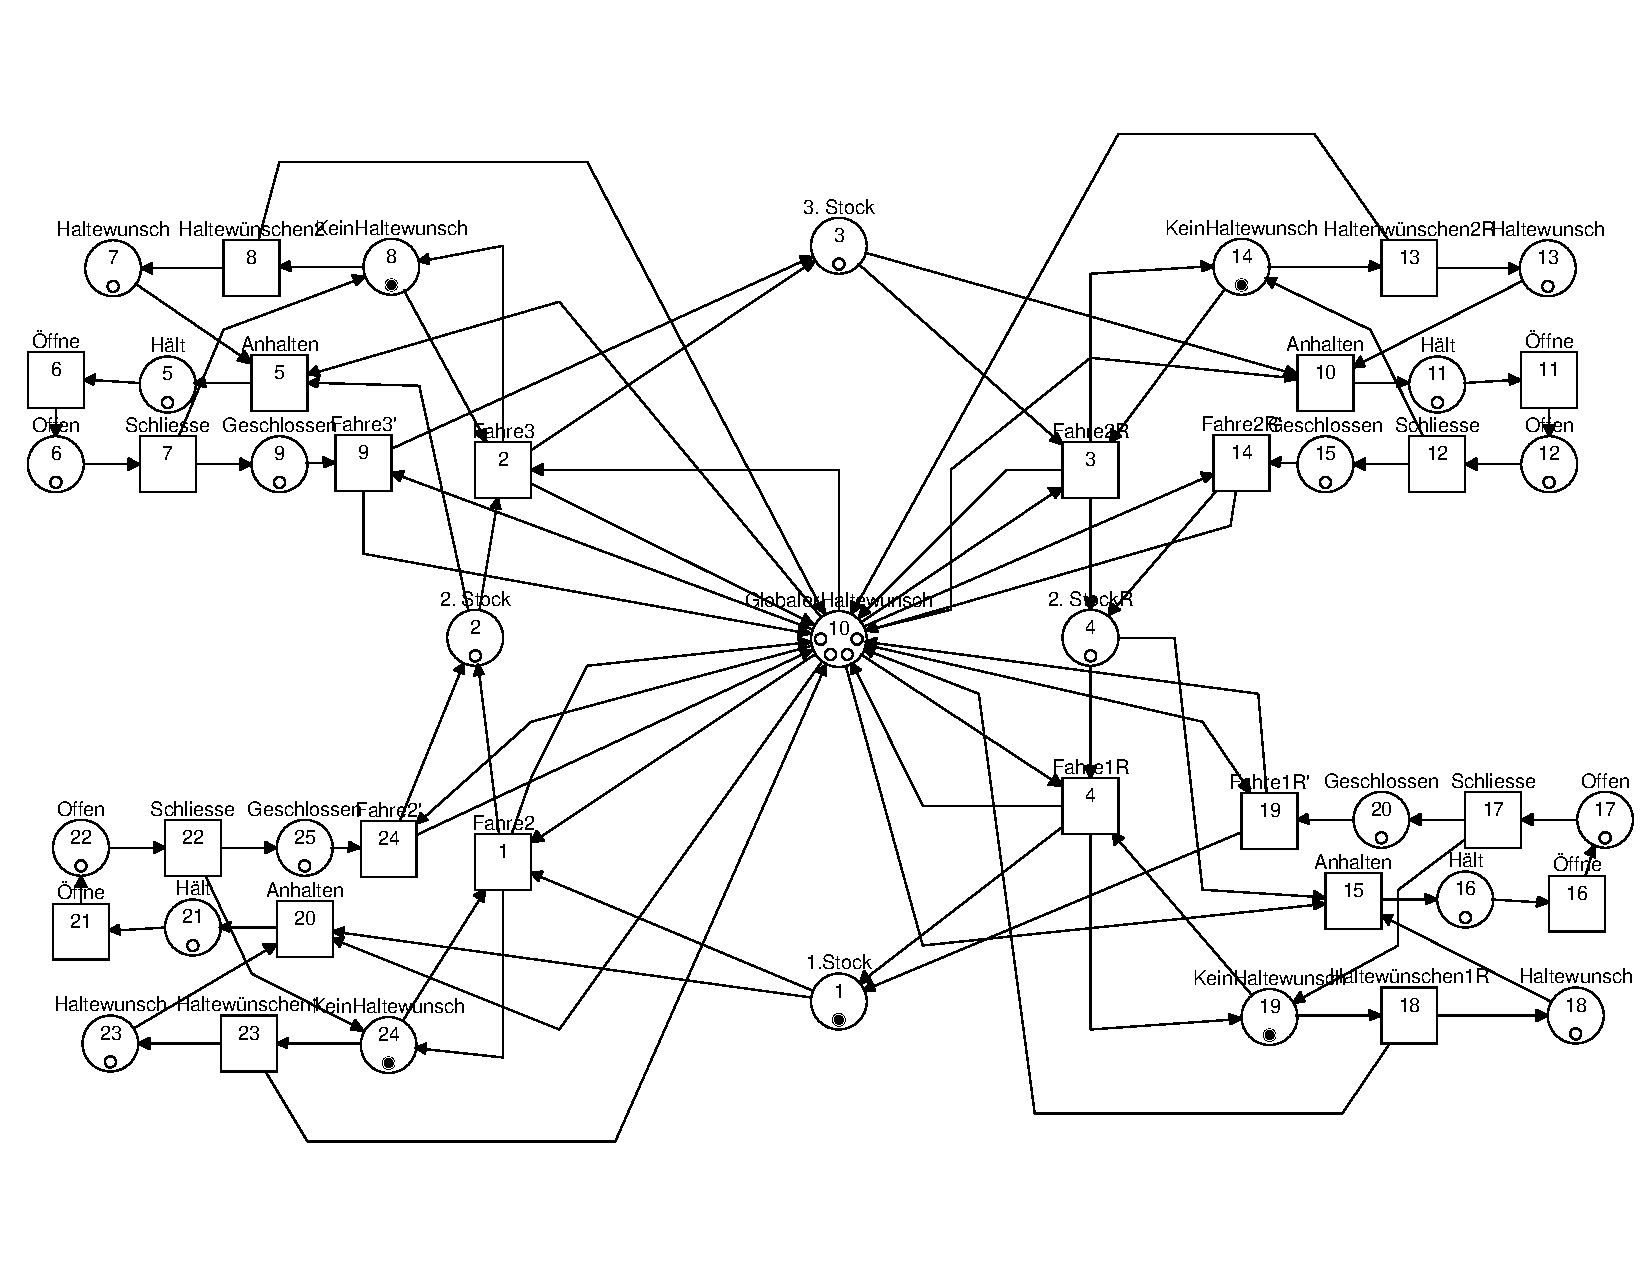
\includegraphics[width=1\textwidth]{prak_aufg3_fertig_bugfix2.pdf}

\item Gebt das Netz formal in klassischer Darstellung an.

$N = (P, T, W, K, M_0)$

$P_1 = \{ Stock_1, Stock_2, Stock_3, Stock_{2R}, GlobalerHaltewunsch \}$

$P_2 = \bigcup_{i \in \{ 1, 2, 2R, 1R \}} \{ Haltewunsch_i, KeinHaltewunsch_i, H"alt_i, Offen_i, Geschlossen_i \}$

$P = P_1 \cup P_2$

Es gelte:

$
Stock_1 < Stock_2 < Stock_3 < Stock_{2R} < GlobalerHaltewunsch < 
Haltewunsch_1 < KeinHaltewunsch_1 < H"alt_1 < Offen_1 < Geschlossen_1 < 
Haltewunsch_2 < KeinHaltewunsch_2 < H"alt_2 < Offen_2 < Geschlossen_2 < 
Haltewunsch_{2R} < KeinHaltewunsch_{2R} < H"alt_{2R} < Offen_{2R} < Geschlossen_{2R} < 
Haltewunsch_{1R} < KeinHaltewunsch_{1R} < H"alt_{1R} < Offen_{1R} < Geschlossen_{1R}
$

$T = \bigcup_{i \in \{ 1, 2, 2R, 1R \}} \{ Fahre_i, Fahre_i', Haltew"unschen_i, Anhalten_i, "Offne_i, Schliesse_i \}$

$
W(x,y) = 1 f"ur (x,y) \in \{
  (Stock_1, Fahre_2), (Stock_1, Anhalten_1), \\
  (Fahre_{1R}, Stock_1), (Fahre_{1R'}, Stock_1), \\
  (KeinHaltewunsch_1, Haltew"unschen_1), (KeinHaltewunsch_1, Fahre_2), \\
  (Fahre_2, KeinHaltewunsch_1), (Schliesse_1, KeinHaltewunsch_1), \\
  (Haltew"unschen_1, Haltewunsch_1), (Haltew"unschen_1, GlobalerHaltewunsch), \\
  (Haltewunsch_1, Anhalten_1), (GlobalerHaltewunsch, Anhalten_1), \\
  (Anhalten_1, H"alt_1), (H"alt_1, "Offne_1), \\
  ("Offne_1, Offen_1), (Offen_1, Schliesse_1), \\
  (Schliesse_1, Geschlossen_1), (Geschlossen_1, Fahre_{2'}), \\
  (Fahre_{2'}, Stock_2), (Fahre_{2'}, GlobalerHaltewunsch), \\
  (GlobalerHaltewunsch, Fahre_{2'}), (Fahre_2, GlobalerHaltewunsch), \\
  (GlobalerHaltewunsch, Fahre_2), (Fahre_2, Stock_2), \\
  (Stock_2, Fahre_3), (Stock_2, Anhalten_2), \\
  (Fahre_3, Stock_3), (KeinHaltewunsch_2, Fahre_3), \\
  (Fahre_3, KeinHaltewunsch_2), (Fahre_3, GlobalerHaltewunsch), \\
  (GlobalerHaltewunsch, Fahre_3), (Fahre_{3'} GlobalerHaltewunsch), \\
  (GlobalerHaltewunsch, Fahre_{3'}), (Fahre_{3'}, Stock_3), \\
  (Geschlossen_2, Fahre_{3'}), (Schliesse_2, Geschlossen_2), \\
  (Offen_2, Schliesse_2), (Schliesse_2, KeinHaltewunsch_2), \\
  ("Offne_2, Offen_2), (H"alt_2, "Offne_2), \\
  (Anhalten_2, H"alt_2), (KeinHaltewunsch_2, Haltew"unschen_2), \\
  (Haltew"unschen_2, Haltewunsch_2), (Haltew"unschen_2, GlobalerHaltewunsch), \\
  (Haltewunsch_2, Anhalten_2), (GlobalerHaltewunsch, Anhalten_2), \\
  (Stock_3, Anhalten_{2R}), (Stock_3, Fahre_{2R}), \\
  (KeinHaltewunsch_{2R}, Haltew"unschen_{2R}), (KeinHaltewunsch_{2R}, Fahre_{2R}), \\
  (Fahre_{2R}, KeinHaltewunsch_{2R}), (Schliesse_{2R}, KeinHaltewunsch_{2R}),\\
  (Haltew"unschen_{2R}, GlobalerHaltewunsch), (Haltew"unschen_{2R}, Haltewunsch_{2R}), \\
  (Haltewunsch_{2R}, Anhalten_{2R}), (Anhalten_{2R}, H"alt_{2R}), \\
  (GlobalerHaltewunsch, Anhalten_{2R}), (H"alt_{2R}, "Offne_{2R}), \\
  ("Offne_{2R}, Offen_{2R}), (Offen_{2R}, Schliesse_{2R}), \\
  (Schliesse_{2R}, Geschlossen_{2R}), (Geschlossen_{2R}, Fahre_{2R'}), \\
  (Fahre_{2R'}, GlobalerHaltewunsch), (GlobalerHaltewunsch, Fahre_{2R'}), \\
  (Fahre_{2R'}, Stock_{2R}), (Fahre_{2R}, GlobalerHaltewunsch), \\
  (GlobalerHaltewunsch, Fahre_{2R}), (Fahre_{2R}, Stock_{2R}), \\
  (Stock_{2R}, Fahre_{1R}), (Stock_{2R}, Anhalten_{1R}), \\
  (Haltewunsch_{1R}, Anhalten_{1R}), (Haltew"unschen_{1R}, Haltewunsch_{1R}), \\
  (Haltew"unschen_{1R}, GlobalerHaltewunsch), (KeinHaltewunsch_{1R}, Haltew"unschen_{1R}), \\
  ("Offne_{1R}, Offen_{1R}), (H"alt_{1R}, "Offne_{1R}), (Offen_{1R}, Schliesse_{1R}), \\
  (Schliesse_{1R}, Geschlossen_{1R}), (Schliesse_{1R}, KeinHaltewunsch_{1R}), \\
  (Anhalten_{1R}, H"alt_{1R}), (GlobalerHaltewunsch, Anhalten_{1R}), \\
  (Geschlossen_{1R}, Fahre_{1R'}), (Fahre_{1R'}, GlobalerHaltewunsch), \\
  (GlobalerHaltewunsch, Fahre_{1R'}), (KeinHaltewunsch_{1R}, Fahre_{1R}) \\
  (Fahre_{1R}, KeinHaltewunsch_{1R}), (GlobalerHaltewunsch, Fahre_{1R}), \\
  (Fahre_{1R}, GlobalerHaltewunsch)
\}
$

$W(x,y) = 0$ sonst

$K : P \rightarrow \mathds{N}_0$

$
K(p) = 
  \begin{cases}
    3, & \text{falls $p \in \{ GlobalerHaltewunsch \}$} \\ 
    1, & \text{sonst} \end{cases}$

$M_0 = (
1, 0, 0, 0, 0, 
0, 1, 0, 0, 0, 
0, 1, 0, 0, 0, 
0, 1, 0, 0, 0, 
0, 1, 0, 0, 0
)$

\item Berechnet formal die Schaltfolge zu einer gegebenen Anfangsmarkierung, die eine Fahrt vom ersten in den dritten Stock beschreibt.

% Anfangsmarkierung

Anfangsmarkierung: 
$M_0 = (
1, 0, 0, 0, 0, 
0, 1, 0, 0, 0, 
0, 1, 0, 0, 0, 
0, 1, 0, 0, 0, 
0, 1, 0, 0, 0
)$

% Haltewünschen_2R soll schalten

\textbf{Vorbereich von $Haltew"unschen_{2R}$}:

\begin{addmargin}[1cm]{0cm}
  $\bullet Haltew"unschen_{2R} = \{ KeinHaltewunsch_{2R} \}$

  $Haltew"unschen_{2R}$ aktiviert, da

  $M(KeinHaltewunsch_{2R}) = 1 \geq W(KeinHaltewunsch_{2R}, Haltew"unschen_{2R})$
\end{addmargin}

\textbf{Nachbereich von $Haltew"unschen_{2R}$}:

\begin{addmargin}[1cm]{0cm}
  $Haltew"unschen_{2R} \bullet = \{ Haltewunsch_{2R}, GlobalerHaltewunsch \}$

  $K(Haltewunsch_{2R}) = 1 \geq 1 = 0 + 1 = M(Haltewunsch_{2R}) + \\ W(Haltew"unschen_{2R}, Haltewunsch_{2R})$

  $K(Globalerhaltewunsch) = 4 \geq 1 = 0 + 1 = M(GlobalerHaltewunsch) + W(Haltew"unschen_{2R}, GlobalerHaltewunsch)$

  $\implies Haltew"unschen_{2R}$ aktiviert
\end{addmargin}

% Folgezustand M1

$M_0 \xrightarrow{Haltew"unschen_{2R}} M_1$

\begin{addmargin}[1cm]{0cm}
  $M_1(GlobalerHaltewunsch) = M_0(GlobalerHaltewunsch) - \\ W(GlobalerHaltewunsch, Haltew"unschen_{2R}) + \\ W(Haltew"unschen_{2R}, GlobalerHaltewunsch) = 0 - 0 + 1 = 1$

  $M_1(KeinHaltewunsch_{2R}) = M_0(KeinHaltewunsch_{2R}) - \\ W(KeinHaltewunsch_{2R}, Haltew"unschen_{2R}) + \\ W(Haltew"unschen_{2R}, KeinHaltewunsch_{2R}) = 1 - 1 + 0 = 0$

  $M_1(Haltewunsch_{2R}) = M_0(Haltewunsch_{2R}) - \\ W(Haltewunsch_{2R}, Haltew"unschen_{2R}) + \\ W(Haltew"unschen_{2R}, Haltewunsch_{2R}) = 0 - 0 + 1 = 1$

  $\implies$ 
  $M_1 = (
  1, 0, 0, 0, 1, 
  0, 1, 0, 0, 0, 
  0, 1, 0, 0, 0, 
  1, 0, 0, 0, 0, 
  0, 1, 0, 0, 0
  )$
\end{addmargin}

% Fahre2 soll schalten

\textbf{Vorbereich von $Fahre_2$}

\begin{addmargin}[1cm]{0cm}
  $\bullet Fahre_2 = \{ GlobalerHaltewunsch, Stock_1, KeinHaltewunsch_1 \}$

  $Fahre_2$ aktiviert, da

  $M(KeinHaltewunsch_1) = 1 \geq W(KeinHaltewunsch_1, Fahre_2) = 1$  

  $M(GlobalerHaltewunsch) = 1 \geq W(GlobalerHaltewunsch, Fahre_2) = 1$

  $M(Stock_1) = 1 \geq W(Stock_1, Fahre_2) = 1$
\end{addmargin}

\textbf{Nachbereich von $Fahre_2$}

\begin{addmargin}[1cm]{0cm}
  $Fahre_2 \bullet = \{ GlobalerHaltewunsch, Stock_2, KeinHaltewunsch_1 \}$

  $K(GlobalerHaltewunsch) = 4 \geq M(GlobalerHaltewunsch) + \\ W(Fahre_2, GlobalerHaltewunsch) = 1 + 1 = 2$ 

  $K(Stock_2) = 1 \geq M(Stock_2) + W(Fahre_2, Stock_2) = 0 + 1 = 1$

  $K(KeinHaltewunsch_1) = 1 \geq M(KeinHaltewunsch_1) - \\ W(KeinHaltewunsch_1, Fahre_2) + \\ W(Fahre_2, KeinHaltewunsch_1) = 1 - 1 + 1$

  $\implies Fahre_2$ aktiviert
\end{addmargin}

% Folgezustand M2

$M_1 \xrightarrow{Fahre_2} M_2$

\begin{addmargin}[1cm]{0cm}
  $M_2(Stock_1) = M_1(Stock_1) - W(Stock_1, Fahre_2) + W(Fahre_2, Stock1) = 1 - 1 + 0 = 0$

  $M_2(GlobalerHaltewunsch) = M_1(GlobalerHaltewunsch) - \\ W(GlobalerHaltewunsch, Fahre_2) + \\ W(Fahre_2, GlobalerHaltewunsch) = 1 - 1 + 1 = 1$

  $M_2(Stock_2) = M_1(Stock_2) - W(Stock_2, Fahre_2) + \\ W(Fahre_2, Stock_2) = 0 - 0 + 1 = 1$

  $M_2(KeinHaltewunsch_1) = M_1(KeinHaltewunsch_1) - \\ W(KeinHaltewunsch_1, Fahre_2) + \\ W(Fahre_2, KeinHaltewunsch_1) = 1 - 1 + 1 = 1$

  $\implies$ 
  $M_2 = (
  0, 1, 0, 0, 1, 
  0, 1, 0, 0, 0, 
  0, 1, 0, 0, 0, 
  1, 0, 0, 0, 0, 
  0, 1, 0, 0, 0
  )$
\end{addmargin}

% Fahre3 soll schalten

\textbf{Vorbereich von $Fahre_3$}

\begin{addmargin}[1cm]{0cm}
  $\bullet Fahre_3 = \{ GlobalerHaltewunsch, Stock_2, KeinHaltewunsch_2 \}$

  $Fahre_2$ aktiviert, da

  $M(KeinHaltewunsch_2) = 1 \geq W(KeinHaltewunsch_2, Fahre_3) = 1$  

  $M(GlobalerHaltewunsch) = 1 \geq W(GlobalerHaltewunsch, Fahre_3) = 1$

  $M(Stock_3) = 1 \geq W(Stock_2, Fahre_3) = 1$
\end{addmargin}

\textbf{Nachbereich von $Fahre_3$}

\begin{addmargin}[1cm]{0cm}
  $Fahre_3 \bullet = \{ GlobalerHaltewunsch, Stock_3, KeinHaltewunsch_2 \}$

  $K(GlobalerHaltewunsch) = 4 \geq M(GlobalerHaltewunsch) + \\ W(Fahre_3, GlobalerHaltewunsch) = 1 + 1 = 2$ 

  $K(Stock_3) = 1 \geq M(Stock_3) + W(Fahre_3, Stock_3) = 0 + 1 = 1$

  $K(KeinHaltewunsch_2) = 1 \geq M(KeinHaltewunsch_2) - \\ W(KeinHaltewunsch_2, Fahre_3) + \\ W(Fahre_3, KeinHaltewunsch_2) = 1 - 1 + 1$

  $\implies Fahre_3$ aktiviert
\end{addmargin}

% Folgezustand M3

$M_2 \xrightarrow{Fahre_3} M_3$

\begin{addmargin}[1cm]{0cm}
  $M_3(Stock_2) = M_2(Stock_2) - W(Stock_2, Fahre_3) + W(Fahre_3, Stock2) = 1 - 1 + 0 = 0$

  $M_3(GlobalerHaltewunsch) = M_2(GlobalerHaltewunsch) - \\ W(GlobalerHaltewunsch, Fahre_3) + \\ W(Fahre_3, GlobalerHaltewunsch) = 1 - 1 + 1 = 1$

  $M_3(Stock_3) = M_1(Stock_3) - W(Stock_3, Fahre_3) + W(Fahre_3, Stock_3) = 0 - 0 + 1 = 1$

  $M_3(KeinHaltewunsch_2) = M_2(KeinHaltewunsch_2) - \\ W(KeinHaltewunsch_2, Fahre_3) + \\ W(Fahre_3, KeinHaltewunsch_2) = 1 - 1 + 1 = 1$

  $\implies$ 
  $M_3 = (
  0, 0, 1, 0, 1, 
  0, 1, 0, 0, 0, 
  0, 1, 0, 0, 0, 
  1, 0, 0, 0, 0, 
  0, 1, 0, 0, 0
  )$
\end{addmargin}

% Anhalten2R soll schalten

\textbf{Vorbereich von $Anhalten_{2R}$}

\begin{addmargin}[1cm]{0cm}
  $\bullet Anhalten_{2R} = \{ Stock_3, GlobalerHaltewunsch, Haltewunsch_{2R} \}$

  $Anhalten_{2R}$ aktiviert, da

  $M(Stock_3) = 1 \geq W(Stock_3, Anhalten_{2R}) = 1$  

  $M(GlobalerHaltewunsch) = 1 \geq W(GlobalerHaltewunsch, Anhalten_{2R}) = 1$

  $M(Haltewunsch_{2R}) = 1 \geq W(Haltewunsch_{2R}, Anhalten_{2R}) = 1$
\end{addmargin}

\textbf{Nachbereich von $Anhalten_{2R}$}

\begin{addmargin}[1cm]{0cm}
  $Anhalten_{2R} \bullet = \{ H"alt_{2R} \}$

  $K(H"alt_{2R}) = 1 \geq M(H"alt_{2R}) + W(Anhalten_{2R}, H"alt_{2R}) = 0 + 1 = 1$

  $\implies Anhalten_{2R}$ aktiviert
\end{addmargin}

$M_3 \xrightarrow{Anhalten_{2R}} M_4$

\begin{addmargin}[1cm]{0cm}
  $M_4(Stock_3) = M_3(Stock_3) - W(Stock_3, Anhalten_{2R}) + W(Anhalten_{2R}, Stock_3) = 1 - 1 + 0 = 0$

  $M_4(GlobalerHaltewunsch) = M_3(GlobalerHaltewunsch) - \\ W(GlobalerHaltewunsch, Anhalten_{2R}) + \\ W(Anhalten_{2R}, GlobalerHaltewunsch) = 1 - 1 + 0 = 0$

  $M_4(Haltewunsch_{2R}) = M_3(Haltewunsch_{2R}) - \\ W(Haltewunsch_{2R}, Anhalten_{2R}) + \\ W(Anhalten_{2R}, Haltewunsch_{2R}) = 1 - 1 + 0 = 0$

  $M_4(H"alt_{2R}) = M_3(H"alt_{2R}) - \\ W(H"alt_{2R}, Anhalten_{2R}) + W(Anhalten_{2R}, H"alt_{2R}) = 0 - 0 + 1 = 1$

  $\implies$ 
  $M_4 = (
  0, 0, 0, 0, 0, 
  0, 1, 0, 0, 0, 
  0, 1, 0, 0, 0, 
  0, 0, 0, 1, 0, 
  0, 1, 0, 0, 0
  )$
\end{addmargin}

Der Aufzug ist nun auf dem 3. Stock und hat angehalten.

\item Gebt den Erreichbarkeitsgraphen grafisch zu einer gegebenen Anfangsmarkierung an.

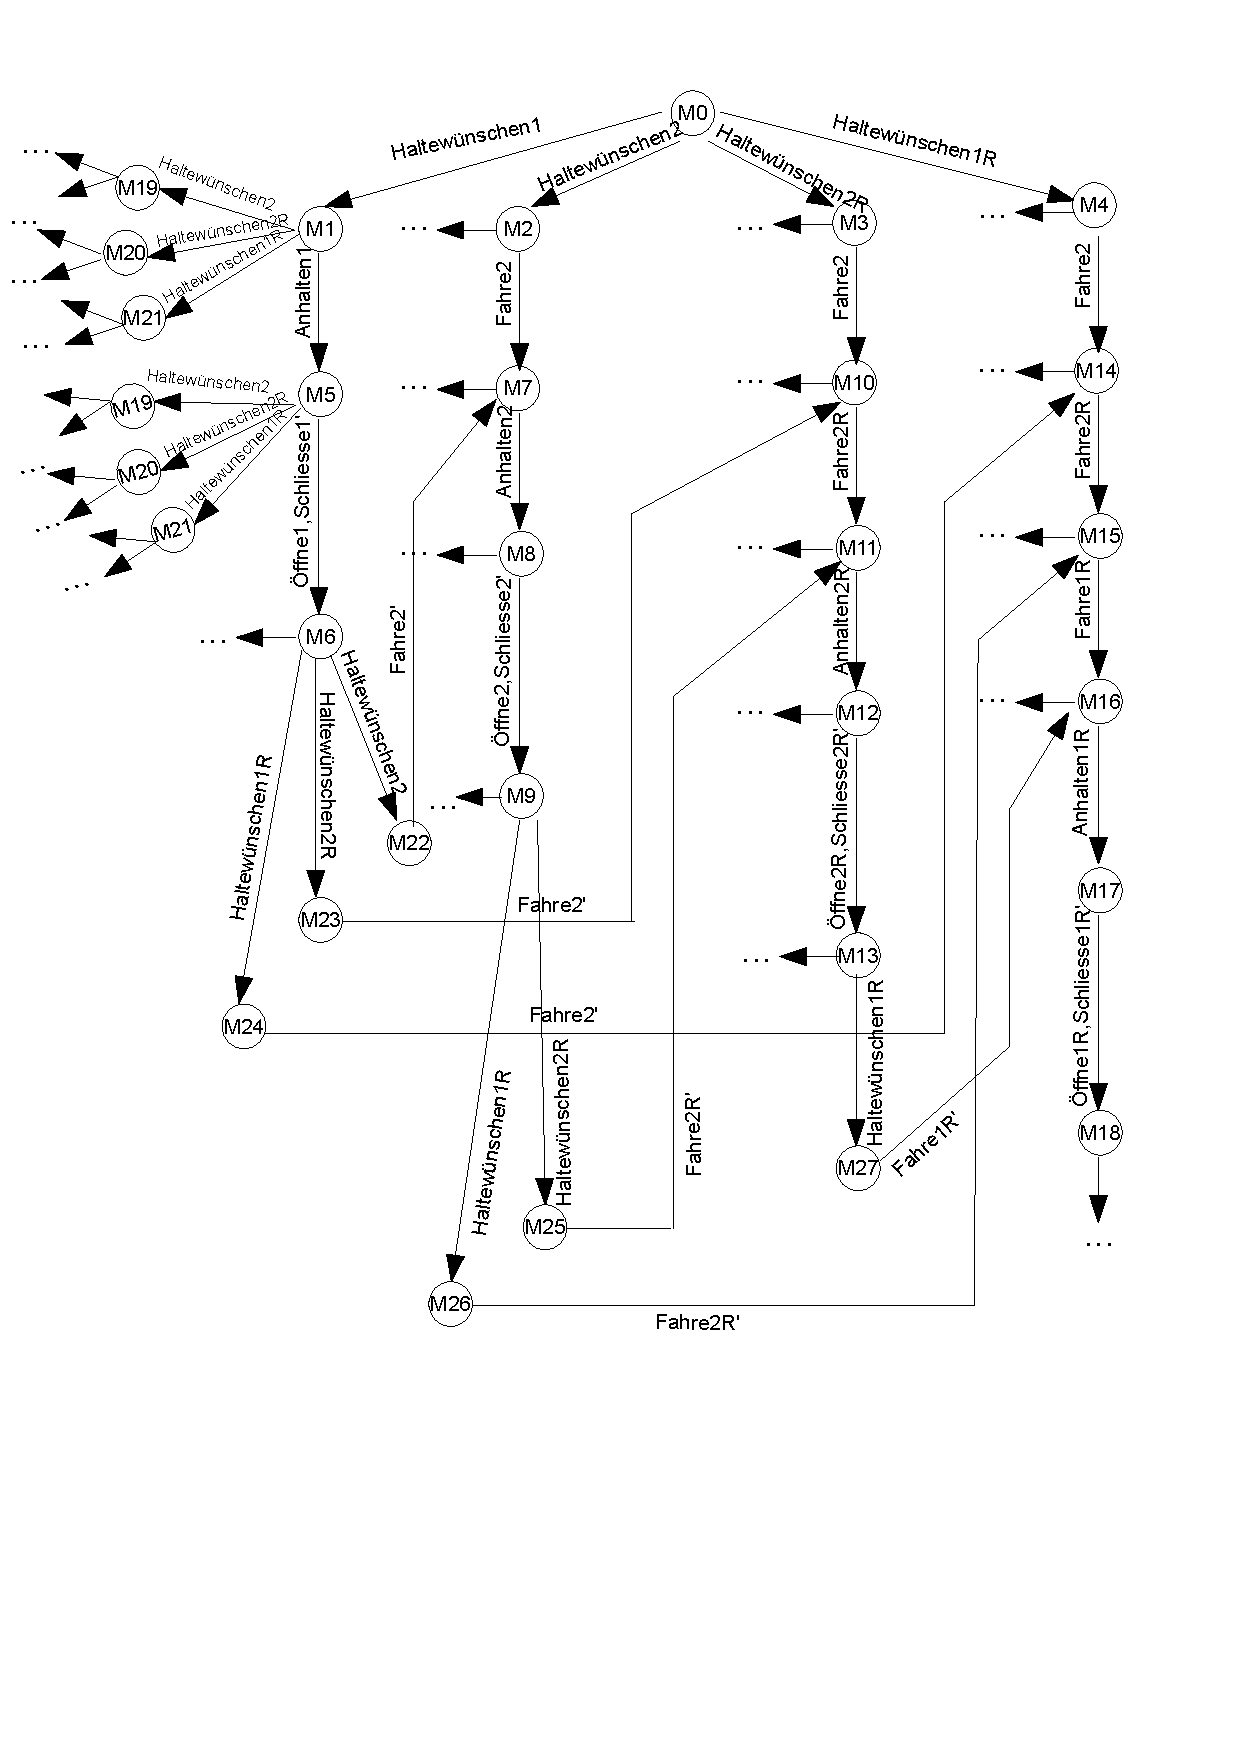
\includegraphics[width=1\textwidth]{eg.pdf}

Gebt das Netzkomplement Eures Netzes formal und grafisch an. Ggf koennt Ihr auch
einen aussagekraeftigen Ausschnitt waehlen, falls das Netz zu gross wird.

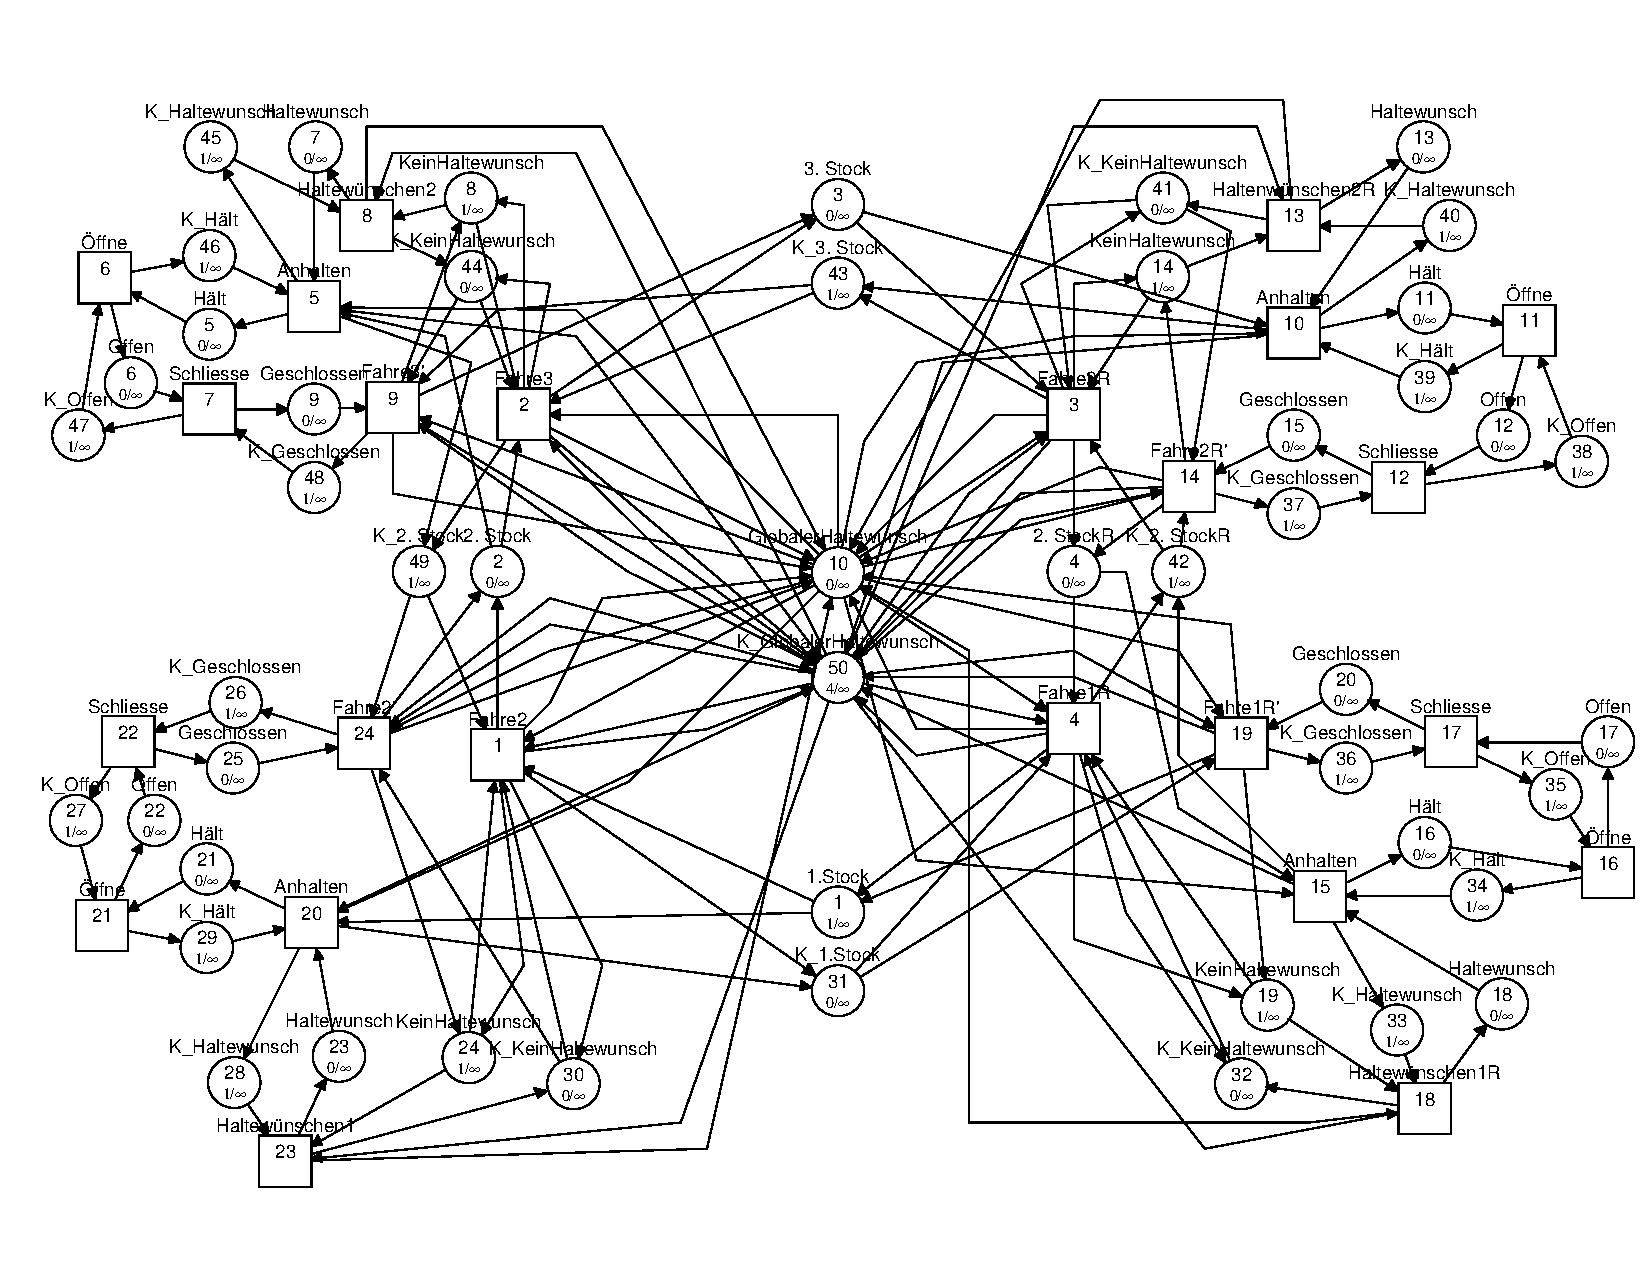
\includegraphics[width=1\textwidth]{prak_aufg3_fertig_bugfix_komplement.pdf}

Formale Beschreibung:\\
$N' = (P',T,W',M_0')\\
P' = P \cup \overline{P}\\
P = siehe oben\\
\overline{P}= \lbrace\overline{1Stock},\overline{2Stock},\overline{3Stock},\overline{2StockR},\\
\overline{Haelt},\overline{Offen},\overline{Haltewunsch},\overline{KeinHaltewunsch},\overline{Geschlossen},\overline{GlobalerHaltewunsch},\\
\overline{Haelt},\overline{Offen},\overline{Haltewunsch},\overline{KeinHaltewunsch},\overline{Geschlossen},\\
\overline{Haelt},\overline{Offen},\overline{Haltewunsch},\overline{KeinHaltewunsch},\overline{Geschlossen},\\
\overline{Haelt},\overline{Offen},\overline{Haltewunsch},\overline{KeinHaltewunsch},\overline{Geschlossen}\rbrace\\
T= \lbrace T1 bis T24 \rbrace\\
W' : (P' \times T) \cup (T \times P') \rightarrow \mathds{N}_0
\forall (x, y) \in (P' \times T) \cup (T \times P'): W'(x,y) = 1\\
M_0' = (
0, 1, 1, 1, 1, 
1, 0, 1, 1, 4, 
1, 0, 1, 1, 1, 
1, 0, 1, 1, 1, 
1, 0, 1, 1, 1
)
$

\end{enumerate}

\end{document}

